\documentclass[aspectratio=169,10pt]{beamer}
\usetheme{Madrid}\usecolortheme{beaver}
\usepackage[utf8]{inputenc}\usepackage[T1]{fontenc}\usepackage{lmodern}
\usepackage[spanish,es-nodecimaldot,es-noquoting]{babel}\spanishplainpercent
\usepackage{amsmath,graphicx,booktabs}
\usepackage[output-decimal-marker={,},group-separator={\,},group-minimum-digits=4,exponent-product=\times,separate-uncertainty=true]{siunitx}
\setbeamertemplate{navigation symbols}{}
\DeclareUnicodeCharacter{2080}{\ensuremath{_0}}\DeclareUnicodeCharacter{2081}{\ensuremath{_1}}
\DeclareUnicodeCharacter{2082}{\ensuremath{_2}}\DeclareUnicodeCharacter{2083}{\ensuremath{_3}}
\DeclareUnicodeCharacter{2070}{\ensuremath{^0}}\DeclareUnicodeCharacter{00B9}{\ensuremath{^1}}
\DeclareUnicodeCharacter{2074}{\ensuremath{^4}}\DeclareUnicodeCharacter{2075}{\ensuremath{^5}}
\DeclareUnicodeCharacter{2076}{\ensuremath{^6}}\DeclareUnicodeCharacter{207B}{\ensuremath{^-}}
\DeclareUnicodeCharacter{03B1}{\ensuremath{\alpha}}\DeclareUnicodeCharacter{03B2}{\ensuremath{\beta}}
\DeclareUnicodeCharacter{03B3}{\ensuremath{\gamma}}\DeclareUnicodeCharacter{03B4}{\ensuremath{\delta}}
\DeclareUnicodeCharacter{03B5}{\ensuremath{\varepsilon}}\DeclareUnicodeCharacter{03B8}{\ensuremath{\theta}}
\DeclareUnicodeCharacter{03BB}{\ensuremath{\lambda}}\DeclareUnicodeCharacter{03BC}{\ensuremath{\mu}}
\DeclareUnicodeCharacter{03BD}{\ensuremath{\nu}}\DeclareUnicodeCharacter{03C0}{\ensuremath{\pi}}
\DeclareUnicodeCharacter{03C1}{\ensuremath{\rho}}\DeclareUnicodeCharacter{03C3}{\ensuremath{\sigma}}
\DeclareUnicodeCharacter{03C4}{\ensuremath{\tau}}\DeclareUnicodeCharacter{03C6}{\ensuremath{\phi}}
\DeclareUnicodeCharacter{03C7}{\ensuremath{\chi}}\DeclareUnicodeCharacter{03C9}{\ensuremath{\omega}}
\DeclareUnicodeCharacter{0394}{\ensuremath{\Delta}}\DeclareUnicodeCharacter{03A3}{\ensuremath{\Sigma}}
\DeclareUnicodeCharacter{2212}{\ensuremath{-}}\DeclareUnicodeCharacter{2248}{\ensuremath{\approx}}
\DeclareUnicodeCharacter{2264}{\ensuremath{\le}}\DeclareUnicodeCharacter{2265}{\ensuremath{\ge}}
\DeclareUnicodeCharacter{2192}{\ensuremath{\to}}\DeclareUnicodeCharacter{27E8}{\ensuremath{\langle}}
\DeclareUnicodeCharacter{27E9}{\ensuremath{\rangle}}\DeclareUnicodeCharacter{2032}{\ensuremath{'}}
\DeclareUnicodeCharacter{2033}{\ensuremath{''}}

\title[Proyecto 19]{Proyecto 19. Acelerador lineal}
\subtitle{Aceleradores}
\author{Jaime A. Betancourt}
\institute{Herramientas Computacionales para la Física --- Proyectos avanzados con Python}
\date{\today}
\begin{document}
\frame{\titlepage}
\begin{frame}{Modelo}
\begin{itemize}
\item $\Delta E=qV\cos\phi$; \ $E_N=E_0+\sum qV_i\cos\phi_i$; \ celdas $L_n=\beta_n\lambda$.
\item Mapa por celda: $T_{i+1}=T_i+qV\cos\phi_i$, \ $\phi_{i+1}=\phi_i+\omega L_i/(\beta c)-2\pi$.
\item Estabilidad para $\phi_s<0$: $\mu^2=2\pi qV(-\sin\phi_s)/(mc^2\beta^2\gamma^3)$.
\end{itemize}
\end{frame}
\begin{frame}{Diseño de las celdas}
\centering
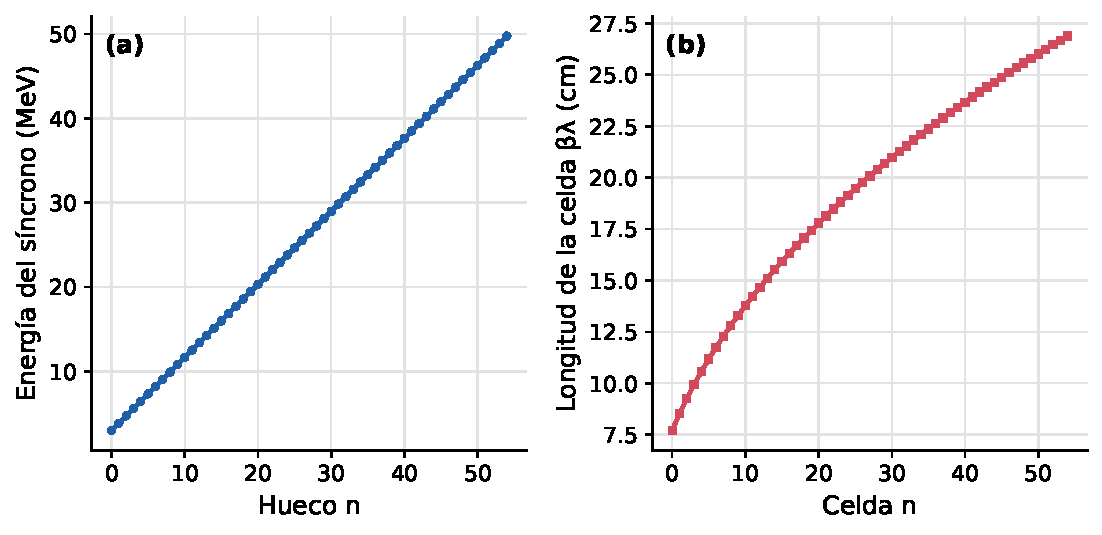
\includegraphics[width=\linewidth,height=0.74\textheight,keepaspectratio]{../figuras/fig01_diseno.pdf}
\end{frame}
\begin{frame}{Espacio de fases}
\centering
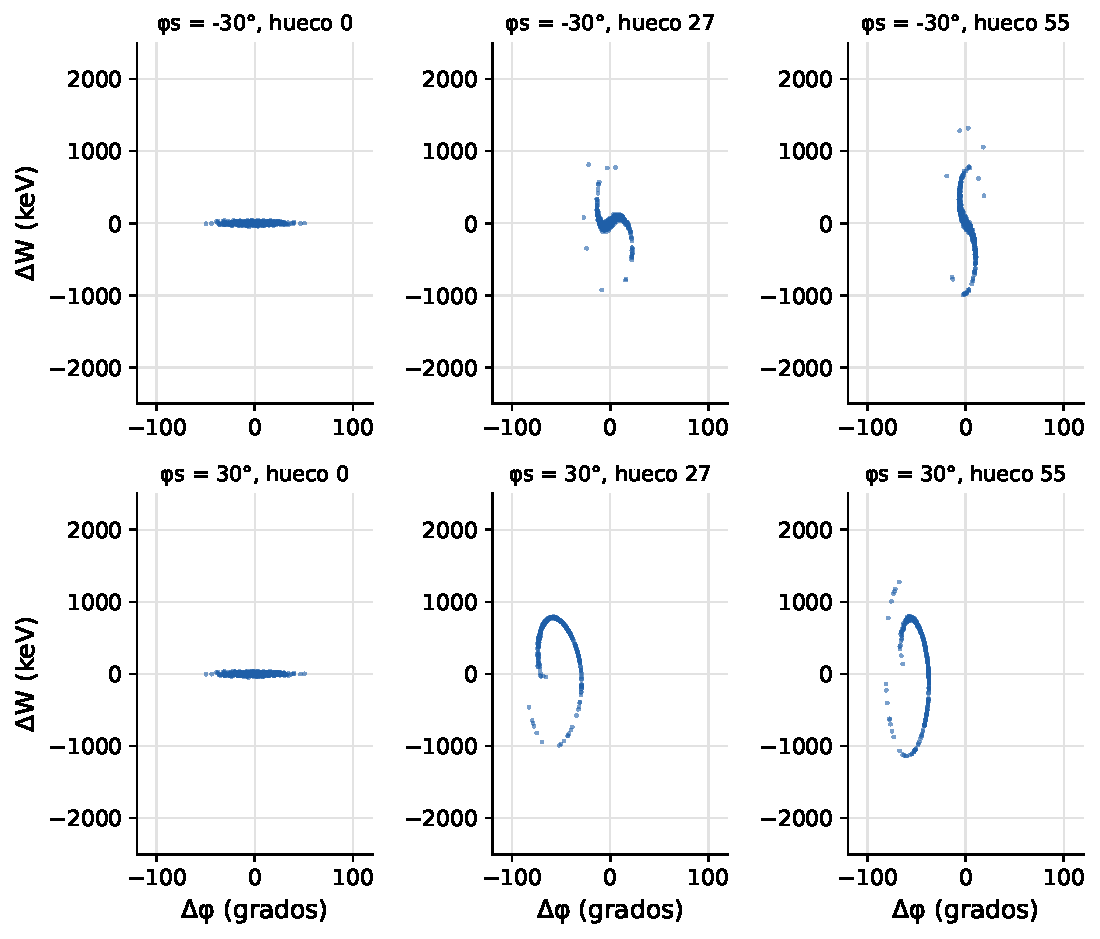
\includegraphics[width=\linewidth,height=0.74\textheight,keepaspectratio]{../figuras/fig02_espacio_fases.pdf}
\end{frame}
\begin{frame}{Oscilaciones de sincrotrón}
\centering
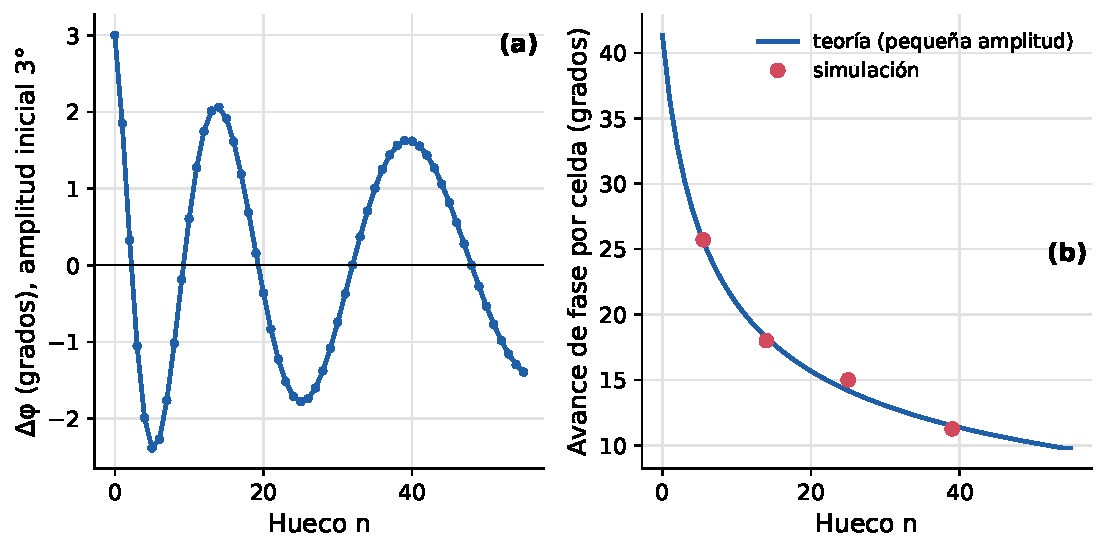
\includegraphics[width=\linewidth,height=0.74\textheight,keepaspectratio]{../figuras/fig03_sincrotron.pdf}
\end{frame}
\begin{frame}{Fase, sincronización y electrones}
\centering
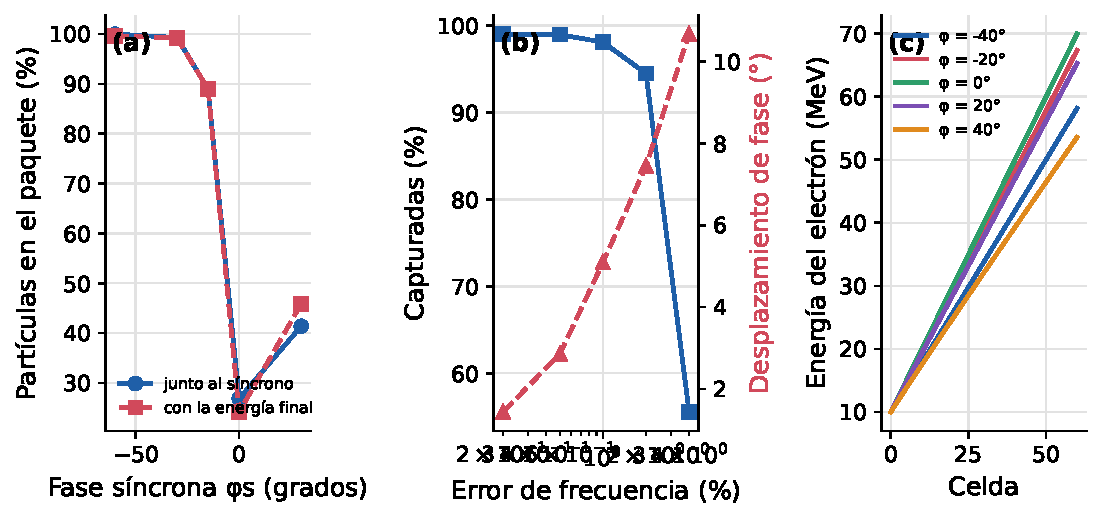
\includegraphics[width=\linewidth,height=0.74\textheight,keepaspectratio]{../figuras/fig04_estabilidad_electrones.pdf}
\end{frame}
\begin{frame}{Conclusiones}
\begin{itemize}
\item \num{3} $\to$ \num{50}~MeV: 55 celdas, \num{10.59}~m.
\item $\phi_s=-30°$: \num{99.3}\,\% agrupado; cresta: \num{24.1}\,\%.
\item Electrones: sin oscilaciones de fase.
\end{itemize}
\end{frame}
\end{document}